\section{MapReduce}


% \begin{figure*}[!h]
%     \centering
%     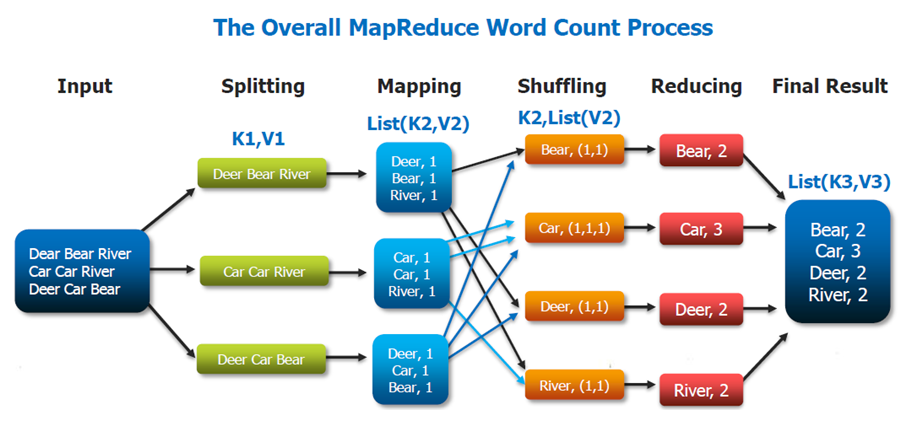
\includegraphics[height=150px]{images/mapreduce.png}
%     \caption{Principe générale du MapReduce}
%     \label{fig: image du site https://www.lebigdata.fr/mapreduce-tout-savoir}
% \end{figure*}

Le MapReduce est un modèle algorithmique conçue comme un outil d’analyse de très grands ensembles de données basé sur le concept de programmation parallèle. Le MapReduce définit un nouveau paradigme, c’est-à-dire une nouvelle façon de penser et de faire qui consiste à découper un problème en tâches. Ce schéma de penser algorithmique découpe le traitement d’un fichier de données en tâches indépendantes suivant deux phases :  
\begin{itemize}
    \item Le Map : qui consiste à transformer les données d’entrée dans des paires clé\textbackslash valeurs
    \item Le Reduce : qui est une fonction de hachage agrégeant toutes les valeurs associées à une même clé. 
\end{itemize}

Il existe une phase qui précède le Map le split pour le découpage des données d’entrée et une phase Intermédier shuffle \& sort entre le Map et le Reduce qui consiste à trier les paires clé\textbackslash valeur générés. Le MapReduce c’est donc ce qui se passe entre la rentrée et la sortie finale. \cite{chokogoue_livre_nodate, sardar_partition_2018}

\subsection{Petite historique} 

Il y a quelques années, google s’est rendu compte qu’il avait un besoin spécifique de traiter l’énorme quantité de données qu’ils avaient. Ces données pouvaient être structurées, semi-structurées ou même non structurées. Ils avaient besoin de nouveaux algorithmes pour pouvoir traiter ces gigantesques volumes de données avec des vitesses d’exécution très rapide voir quasi-instantané. Pour cela, ils mirent en place des équipes de recherche ce qui déboucha sur le développement de deux nouvelles technologies différentes de tous ce qui existaient au paravent 

Il s’agit :  
\begin{itemize}
    \item Du stockage distribué des données avec le GFS 
    \item Du paradigme de traitement sur ces données (MapReduce)  
\end{itemize}

Après cela, Google publia ses recherches dans un article qui présentait son algorithme basé sur des opérations analytiques à grandes échelle sur un grand cluster de serveurs. Ses travaux sont toujours disponibles à l’adresse \url{http://research.google.com/archive/mapreduce.html} 

A cette époque, Doug Cutting, employé chez Google et bénévole pour Apache Lucene, se rend compte qu’il a des besoins similaires. Il lit les travaux de recherche s’approprie les concepts et décidé alors d’implémenter sa propre version Open Source qui deviendra Hadoop. Il s’inspira du doudou de son fils alors âgé de cinq ans, pour le logo et le nom de ce nouveau Framework
.
\subsection{Principe général du MapReduce}
Le MapReduce est un modèle algorithmique comportant
deux phases (le Map et le Reduce), quatre si l’on considère (le slipt et le shuflle \& sort) permettant de paralléliser le traitement :
 

\begin{itemize}
    \item \emph{phase Map} : Cette phase Map, transforme les données d’entrées en de paires clé\textbackslash valeur. Les clés générées ne le sont pas au sens des “clés primaire” comme pour les bases de données. Elles ne sont pas uniques, ce sont juste des identifiants arbitraires qui sont affectés aux valeurs des paires. Cependant, pour toutes les valeurs identiques, on affecte une même clé.

    \item \emph{phase shuffle\& sort} :  Pour cette phase, il s’agit d’une part à trier par clé toutes les paires clé\textbackslash valeur générées lors de la phase Map et d’autre part à regrouper dans une liste, pour chaque clé, l’ensemble de ses valeurs.

    \item \emph{pahse Reduce} :  Le but de cette phase est d’agréger les valeurs des clés reçus par le Shuffle. C’est l’utilisateur qui définit qu’elle fonction d’agrégat il souhaite utiliser soit la somme, le comptage ou même l’envoie à un autre job MapReduce. 

\end{itemize}

% L’exemple \ref{fig: image du site https://www.lebigdata.fr/mapreduce-tout-savoir} illustre parfaitement les différentes phases avec un exemple ou il faut compter le nombre d’occurrences pour chaque mot.
